\chapter{JENIS-JENIS PAKET DATA}

\begin{enumerate}[A.]

  \item \textbf{\textit{Financial Transaction}}
  
  Gambaran mengenai data elemen yang disertakan dalam paket data SPOPD untuk jenis paket data \textit{Financial Transaction Request} dapat dilihat pada tabel \ref{tab:fin-trans}.
  
\begin{table}[H]
  \centering
  \scriptsize
  \begin{tabular}{|p{3em}|p{10em}|p{3em}|p{3em}|l|l|}
  \hline
  \multicolumn{2}{|c|}{\textbf{Data Element}} & \multicolumn{2}{|p{6em}|}{\textbf{Klasifikasi Paket Data}} & \multirow{2}{*}{\textbf{Format}} & \multirow{2}{*}{\textbf{Attr}} \\
  \cline{1-4}
  \textbf{Bit Map} & \textbf{Deskripsi} & \textbf{Req} & \textbf{Res} &  & \\
  \hline
  \hline
  & Message Type & 0200 & 0210 & & \\
  \hline
  & Primary Bit Map & M & M & & B64 \\
  \hline
  P-2 & Primary Account Number & M & M & LLVAR & N..16 \\
  \hline
  P-3 & Processing Code & M & M & & N6 \\
  \hline
  P-4 & Transaction Amount & M & M & & N12 \\
  \hline
  P-7 & Transmission Date and Time & M & M & MMDDhhmmss & N10 \\
  \hline
  P-11 & System Trace Audit Number & M & M & & N6 \\
  \hline
  P-12 & Local Transaction Time & M & M & hhmmss & N6 \\
  \hline
  P-13 & Local Transaction Date & M & M & MMDD & N4 \\
  \hline
  P-18 & Merchant Type (Kode Produksi) & M & M & & N4 \\
  \hline
  P-32 & Acquiring Institution Identification Code & M & M & LLVAR & N4 \\
  \hline
  P-37 & Retrieval Reference Number & M & M & & AN12 \\
  \hline
  P-39 & Response Code & & M & & N2 \\
  \hline
  P-41 & Card Acceptor Terminal Identification & M & M & & AN16 \\
  \hline
  P-48 & Additional Data & M & M & LLLVAR & ANS..210 \\
  \hline
  P-49 & Transaction Currency Code & M & M & & N3 \\
  \hline
  P-63 & Reserved Private & M & M & LLLVAR & N..2 \\
  \hline
  \end{tabular}
  \caption{Tabel Referensi Untuk \textit{Financial Transaction}}
  \label{tab:fin-trans}
\end{table}
  
  \item \textbf{\textit{Reversal Message}}
  
  Gambaran mengenai data elemen yang disertakan dalam paket data SPOPD untuk jenis paket data \textit{Reversal} dapat dilihat pada tabel \ref{tab:reversal}
  
  \begin{table}[H]
    \centering
    \scriptsize
    \begin{tabular}{|p{3em}|p{10em}|p{3em}|p{3em}|l|l|}
    \hline
    \multicolumn{2}{|p{13em}|}{\textbf{Data Element}} & \multicolumn{2}{|p{6em}|}{\textbf{Klasifikasi Paket Data}} & \multirow{2}{*}{\textbf{Format}} & \multirow{2}{*}{\textbf{Attr}} \\
    \cline{1-4}
    \textbf{Bit Map} & \textbf{Deskripsi} & \textbf{Req} & \textbf{Res} & & \\
    \hline
    \hline
    & Message Type & 0400 / 0401 & 0410 / 0411 & & \\
    \hline
    & Primary Bit Map & M & M & & B64 \\
    \hline
    P-1 & Secondary Bit Map & M & M & & B64 \\
    \hline
    P-2 & Primary Account Number & M & M & LLVAR & N..16 \\
    \hline
    P-3 & Processing Code & M & M & & N6 \\
    \hline
    P-4 & Transaction Amount & M & M & & N12 \\
    \hline
    P-7 & Transmission Date and Time & M & M & MMDDhhmmss & N10 \\
    \hline
    P-11 & System Trace Audit Number & M & M & & N6 \\
    \hline
    P-12 & Local Transaction Time & M & M & hhmmss & N6 \\
    \hline
    P-13 & Local Transaction Date & M & M & MMDD & N4 \\
    \hline
    P-18 & Merchant Types (Kode Produksi) & M & M & & N4 \\
    \hline
    P-32 & Acquiring Institution Identification Code & M & M & LLVAR & N4 \\
    \hline
    P-37 & Retrieval Reference Number & M & M & & AN12 \\
    \hline
    P-39 & Response Code & & M & & N2 \\
    \hline
    P-41 & Card Acceptor Terminal Identification & M & M & & AN16 \\
    \hline
    P-48 & Additional Data & M & M & LLLVAR & ANS..210 \\
    \hline
    P-49 & Transaction Currency Code & M & M & & N3 \\
    \hline
    P-63 & Reserved Private & M & M & LLLVAR & N..2 \\
    \hline
    S-90 & Original Data Element & M & M & & N73 \\
    \hline
    \end{tabular}
    \caption{Tabel Referensi Untuk Paket Data \textit{Reversal}}
    \label{tab:reversal}
  \end{table}
  
  \item \textbf{\textit{Network Management Message}}
  
  Gambaran mengenai data elemen yang disertakan dalam paket data SPOPD untuk jenis paket data \textit{Network Management} seperti pada tabel \ref{tab:net-manage}
  
  \begin{table}[H]
    \scriptsize
    \centering
    \begin{tabular}{|p{3em}|p{10em}|p{3em}|p{3em}|l|l|}
      \hline
      \multicolumn{2}{|p{13em}|}{\textbf{Data Element}} & \multicolumn{2}{|p{6em}|}{\textbf{Klasifikasi Paket Data}} & \multirow{2}{*}{\textbf{Format}} & \multirow{2}{*}{\textbf{Attr}} \\
      \cline{1-4}
      \textbf{Bit Map} & \textbf{Deskripsi} & \textbf{Req} & \textbf{Res} & & \\
      \hline
      \hline
      & Message Type & 0800 & 0810 & & \\
      \hline
      & Primary Bit Map & M & M & & B64 \\
      \hline
      P-1 & Secondary Bit Map & M & M & & B64 \\
      \hline
      P-7 & Transmission Date and Time & M & M & MMDDhhmmss & N10 \\
      \hline
      P-11 & System Trace Audit Number & M & M & & N6 \\
      \hline
      P-39 & Response Code & & M & & N2 \\
      \hline
      S-70 & Network Management Information Code & M & M & & N3 \\
      \hline
    \end{tabular}
    \caption{Tabel Referensi Untuk Paket Data \textit{Network Management}}
    \label{tab:net-manage}
  \end{table}

\end{enumerate}

Sedangkan untuk paket data yang dikirimkan oleh Sistem Bank/Tempat Pembayaran ke SPOPD memiliki kejadian alur paket data \textit{request}, \textit{reversal}, dan \textit{timeout} seperti berikut ini :

\begin{itemize}

  \item \textbf{\textit{Paket Data Request}}
  
  Gambaran bagaimana sebuah sistem Bank / Tempat Pembayaran menerima transaksi dan kemudian mengirimkannya ke SPOPD untuk memperoleh pengesahan dapat dilihat pada gambar \ref{fig:data-request}
  
  \begin{figure}[H]
    \centering
    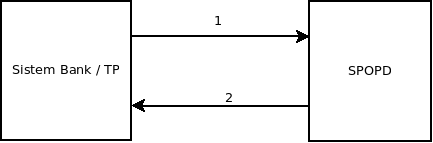
\includegraphics[width=1\textwidth]{./resources/dia-data-request}
    \caption{Skema Data Request PBB-P2}
    \label{fig:data-request}
  \end{figure}
  
  \begin{enumerate}[1.]
    \item Sistem Bank mengirimkan paket data 0200 ke SPOPD untuk mendapatkan pengesahan.
    \item SPOPD melakukan pengesahan terhadap transaksi yang diterima, dan mengirimkan paket data 0210 ke sistem Bank.
  \end{enumerate}
  
  \item \textbf{\textit{Paket Data Reversal}}
  
  Bilamana perangkat ATM, Terminal Teller, atau \textit{channel} lainnya yang dihubungkan ke jaringan Sistem Bank, gagal menyelesaikan sebuah transaksi yang telah disahkan oleh SPOPD, maka sebuah paket reversal harus dikirimkan ke SPOPD. Diagram pada gambar \ref{fig:proses-reversal} memberikan penjelasan bagaimana kejadian tersebut berlangsung :
  
  \begin{figure}[H]
    \centering
    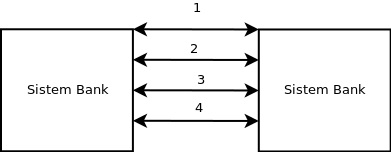
\includegraphics[width=1\textwidth]{./resources/dia-reversal}
    \caption{Skema Data Reversal PBB-P2}
    \label{fig:proses-reversal}
  \end{figure}
  
  \begin{enumerate}[1.]
    \item Sistem Bank mengirimkan paket 0200 ke SPOPD untuk mendapatkan pengesahan.
    \item SPOPD melakukan pengesahan terhadap transaksi yang diterima, dan mengirimkan paket data 0210 ke sistem Bank.
    \item Sistem Bank tidak dapat menindak lanjuti transaksi yang telah disahkan tersebut. Sistem Bank akan mencatat pada basisdatanya sebuah paket data 0400 yang kemudian akan dikirim ke SPOPD pada saat proses Store-and-Forward dilakukan.
    \item SPOPD akan mengirimkan paket data 0410.
  \end{enumerate}
  
  \item \textbf{\textit{Timeout}}
  
  \item \textbf{\textit{Paket Data Network Management}}
  
  \begin{itemize}
    \item \textbf{\textit{Logon/echo-test dikirimkan oleh Sistem Bank/TP}}
    \item \textbf{\textit{Logoff dikirimkan oleh Sistem Bank/TP}}
  \end{itemize}

\end{itemize}